\documentclass[aspectratio=169]{beamer}

\usepackage[T1]{fontenc}
\usepackage[utf8]{inputenc}
\usepackage{lmodern}
\usepackage{microtype}
\usepackage{xcolor}
\usepackage{tikz}
\usetikzlibrary{positioning, arrows.meta}
\usepackage{booktabs}
\usepackage{fontawesome5}

\definecolor{wurgreen}{HTML}{34B233}
\definecolor{darkgreen}{HTML}{1F6B1E}
\definecolor{darknavy}{HTML}{1A1A2E}
\definecolor{midgray}{HTML}{6B7280}
\definecolor{lightgray}{HTML}{F3F4F6}
\definecolor{lightgreen}{HTML}{E8F7E8}
\definecolor{bodytext}{HTML}{1F2937}
\definecolor{warnred}{HTML}{FEE2E2}
\definecolor{warnborder}{HTML}{EF4444}

\usetheme{default}
\usecolortheme{default}
\usefonttheme{professionalfonts}
\setbeamertemplate{navigation symbols}{}
\setbeamertemplate{itemize items}{\textcolor{wurgreen}{\textbullet}}
\setbeamertemplate{itemize subitem}{\textcolor{midgray}{--}}
\setbeamercolor{frametitle}{fg=white, bg=darknavy}
\setbeamerfont{frametitle}{size=\large, series=\bfseries}
\setbeamertemplate{frametitle}{%
  \begin{beamercolorbox}[wd=\paperwidth, ht=1.1cm, dp=0.2cm, leftskip=0.6cm]{frametitle}
    \usebeamerfont{frametitle}\insertframetitle
  \end{beamercolorbox}}
\setbeamercolor{background canvas}{bg=white}
\setbeamercolor{normal text}{fg=bodytext}
\setbeamertemplate{footline}{%
  \begin{beamercolorbox}[wd=\paperwidth, ht=0.4cm, dp=0.15cm]{footline}
    \hspace{0.5cm}\textcolor{midgray}{\tiny Bags, Vectors \& Transformers · Wageningen University \& Research}%
    \hfill\textcolor{midgray}{\tiny \insertframenumber}\hspace{0.4cm}
  \end{beamercolorbox}}

\begin{document}

% ── TITLE SLIDE ──────────────────────────────────────────────────────────────
{
\setbeamertemplate{footline}{}
\begin{frame}[plain]
  \begin{tikzpicture}[remember picture, overlay]
    \fill[darknavy] (current page.south west) rectangle (current page.north east);
    \fill[wurgreen] (current page.south west) rectangle
      ([xshift=0.45cm]current page.north west);
    \node[anchor=west, text=white, font=\huge\bfseries, text width=13cm]
      at ([xshift=1.1cm, yshift=1.2cm]current page.west)
      {Bags, Vectors \& Transformers};
    \node[anchor=west, text=wurgreen, font=\large, text width=12cm]
      at ([xshift=1.1cm, yshift=0.05cm]current page.west)
      {Bias, Measurement \& What Comes Next · Day 2, Part 3};
    \node[anchor=west, text=midgray, font=\small, text width=12cm]
      at ([xshift=1.1cm, yshift=-1.5cm]current page.west)
      {Denise J. Roth, PhD Candidate\\
       Strategic Communication Group · Wageningen University \& Research};
  \end{tikzpicture}
\end{frame}
}

% ── SLIDE 1: Welcome back from notebook ──────────────────────────────────────
\begin{frame}{Welcome Back}
\vspace{0.2cm}
{\small You have now worked with real embeddings: nearest neighbors, analogies, your own
Word2Vec model. This part steps back to ask the questions that matter most for
\textbf{research}:}

\medskip
\begin{itemize}\setlength\itemsep{8pt}
  \item[\textcolor{wurgreen}{\faExclamationTriangle}]
    What do embeddings absorb from their training data --- and why should we worry?
  \item[\textcolor{wurgreen}{\faChartLine}]
    How can that same property be turned into a \textbf{measurement tool} for social science?
  \item[\textcolor{wurgreen}{\faBalanceScale}]
    How do we use embeddings \textbf{responsibly} --- validation and pitfalls?
  \item[\textcolor{wurgreen}{\faArrowRight}]
    Where do static embeddings fall short, and what comes next?
\end{itemize}

\medskip
{\small\textcolor{midgray}{\textit{Did anyone's analogy in the notebook return something
\emph{odd}? Let's start there.}}}
\end{frame}

% ── SLIDE 2: Bias - the finding ──────────────────────────────────────────────
\begin{frame}{Embeddings Absorb Bias}
\vspace{0.2cm}
{\small You may have seen it yourself in the notebook: some analogies return
\textbf{stereotyped} results.}

\medskip
\begin{center}
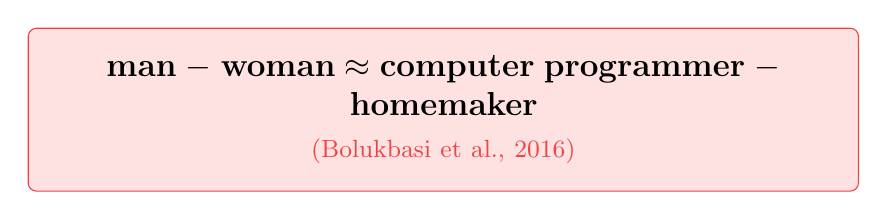
\begin{tikzpicture}
  \node[fill=warnred, draw=warnborder, rounded corners=3pt,
        inner xsep=12pt, inner ysep=10pt, text width=0.8\textwidth]{%
    {\centering\large \textbf{man} $-$ \textbf{woman} $\approx$
    \textbf{computer programmer} $-$ \textbf{homemaker}\par}
    \vspace{4pt}
    {\centering\small\textcolor{warnborder}{(Bolukbasi et al., 2016)}\par}};
\end{tikzpicture}
\end{center}

\bigskip
{\small This is not a bug in the algorithm. Embeddings faithfully learn the
\textbf{statistical patterns} in their training text --- and human text is full of
\textbf{social bias}. The geometry encodes it: gender, race, age, and more.}

\medskip
{\small\textcolor{midgray}{\textit{If you use off-the-shelf embeddings in a pipeline, these
biases ride along silently.}}}
\end{frame}

% ── SLIDE 3: Bias - why it matters ───────────────────────────────────────────
\begin{frame}{Why Bias Matters --- Two Faces}
\vspace{0.3cm}
\begin{columns}[T]
  \column{0.48\textwidth}
  \vspace{0pt}
  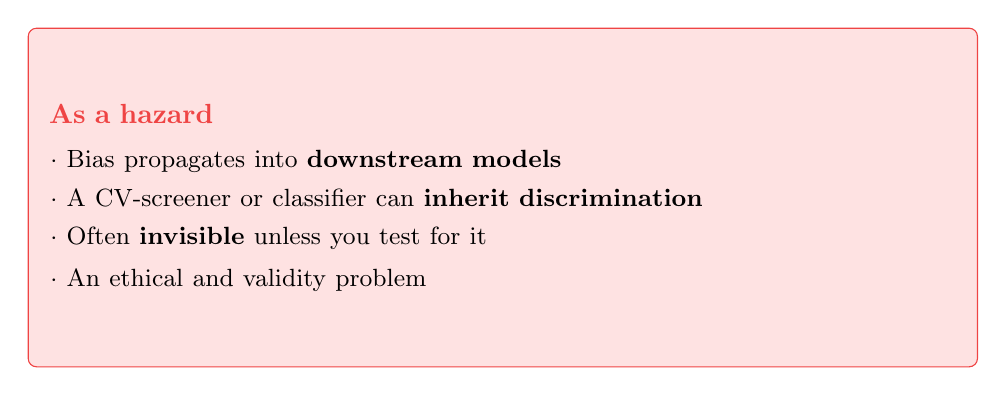
\begin{tikzpicture}
    \node[fill=warnred, draw=warnborder, rounded corners=3pt,
          inner xsep=8pt, inner ysep=8pt, text width=\columnwidth-18pt, minimum height=4.3cm]{%
      \textcolor{warnborder}{\textbf{As a hazard}}\\[5pt]
      {\small
      $\cdot$ Bias propagates into \textbf{downstream models}\\[3pt]
      $\cdot$ A CV-screener or classifier can \textbf{inherit discrimination}\\[3pt]
      $\cdot$ Often \textbf{invisible} unless you test for it\\[3pt]
      $\cdot$ An ethical and validity problem}};
  \end{tikzpicture}

  \column{0.48\textwidth}
  \vspace{0pt}
  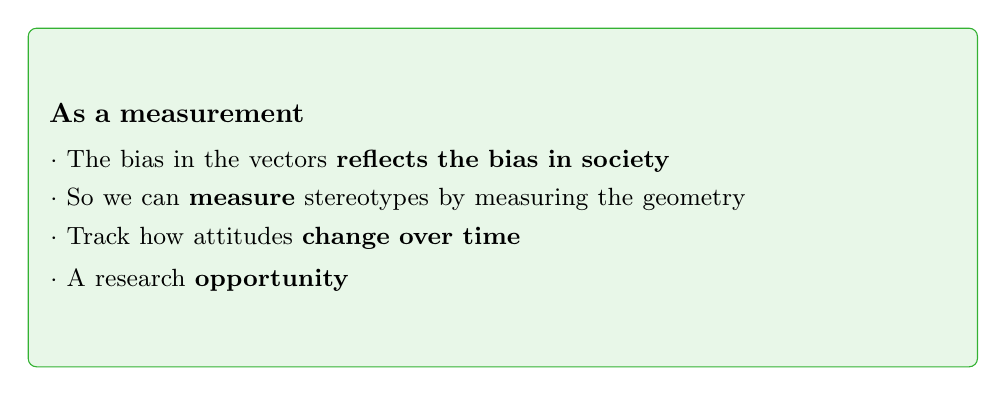
\begin{tikzpicture}
    \node[fill=lightgreen, draw=wurgreen, rounded corners=3pt,
          inner xsep=8pt, inner ysep=8pt, text width=\columnwidth-18pt, minimum height=4.3cm]{%
      \textbf{As a measurement}\\[5pt]
      {\small
      $\cdot$ The bias in the vectors \textbf{reflects the bias in society}\\[3pt]
      $\cdot$ So we can \textbf{measure} stereotypes by measuring the geometry\\[3pt]
      $\cdot$ Track how attitudes \textbf{change over time}\\[3pt]
      $\cdot$ A research \textbf{opportunity}}};
  \end{tikzpicture}
\end{columns}

\medskip
{\small\textcolor{midgray}{\textit{Same fact, two uses. The rest of this section leans into
the second --- embeddings as a lens on society.}}}
\end{frame}

% ── SLIDE 4: Embeddings as measurement ───────────────────────────────────────
\begin{frame}{Embeddings as Measurement}
\vspace{0.2cm}
{\small A powerful idea for social science: if meaning is geometry, then \textbf{social
meaning} is geometry too. We can \textbf{quantify} associations that would be hard to
measure otherwise.}

\medskip
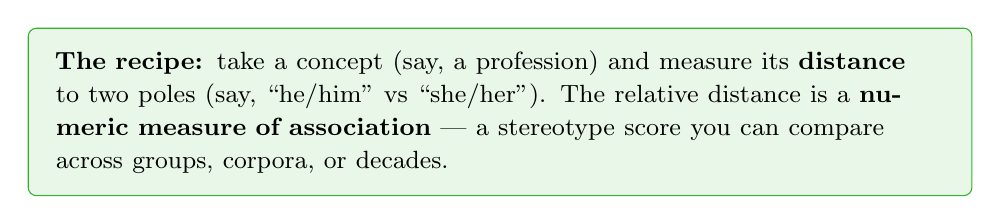
\begin{tikzpicture}
  \node[fill=lightgreen, draw=wurgreen, rounded corners=3pt,
        inner xsep=10pt, inner ysep=8pt, text width=\textwidth-24pt]{%
    {\small \textbf{The recipe:} take a concept (say, a profession) and measure its
    \textbf{distance} to two poles (say, ``he/him'' vs ``she/her''). The relative distance is
    a \textbf{numeric measure of association} --- a stereotype score you can compare across
    groups, corpora, or decades.}};
\end{tikzpicture}

\medskip
\begin{columns}[T]
  \column{0.48\textwidth}
  \vspace{0pt}
  {\small\textbf{Example studies:}}\\[3pt]
  {\small
  \textcolor{wurgreen}{$\cdot$} Garg et al.\ (2018): 100 years of gender \& ethnic stereotypes\\[3pt]
  \textcolor{wurgreen}{$\cdot$} Kozlowski et al.\ (2019): ``the geometry of culture'' --- class, gender, race}

  \column{0.48\textwidth}
  \vspace{0pt}
  {\small\textbf{What you can study:}}\\[3pt]
  {\small
  \textcolor{wurgreen}{$\cdot$} Framing of groups in the news\\[3pt]
  \textcolor{wurgreen}{$\cdot$} Change in public discourse over time\\[3pt]
  \textcolor{wurgreen}{$\cdot$} Cross-national or cross-corpus comparison}
\end{columns}
\end{frame}

% ── SLIDE 5: Measurement - how over time ─────────────────────────────────────
\begin{frame}{Measuring Change Over Time}
\vspace{0.2cm}
{\small The trick that makes this powerful for social science: train (or obtain) \textbf{separate
embeddings for different time periods}, then track how a word's associations \textbf{move}.}

\medskip
\begin{center}
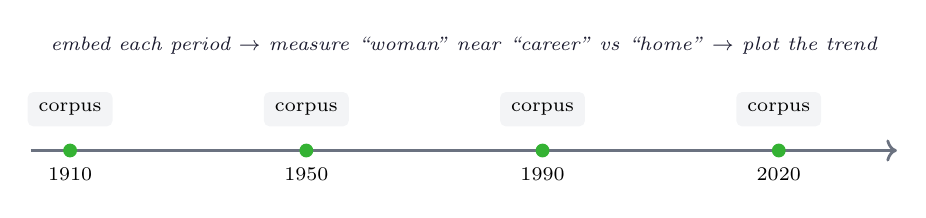
\begin{tikzpicture}[font=\small]
  \draw[->, midgray, line width=1pt] (0,0) -- (11,0);
  \foreach \x/\yr in {0.5/1910, 3.5/1950, 6.5/1990, 9.5/2020} {
    \fill[wurgreen] (\x,0) circle (2.5pt);
    \node[below, font=\scriptsize] at (\x,-0.1) {\yr};
  }
  \node[fill=lightgray, rounded corners=2pt, inner sep=4pt, above, font=\scriptsize] at (0.5,0.3) {corpus};
  \node[fill=lightgray, rounded corners=2pt, inner sep=4pt, above, font=\scriptsize] at (3.5,0.3) {corpus};
  \node[fill=lightgray, rounded corners=2pt, inner sep=4pt, above, font=\scriptsize] at (6.5,0.3) {corpus};
  \node[fill=lightgray, rounded corners=2pt, inner sep=4pt, above, font=\scriptsize] at (9.5,0.3) {corpus};
  \node[text=darknavy, above, font=\scriptsize\itshape] at (5.5,1.1)
    {embed each period $\rightarrow$ measure ``woman'' near ``career'' vs ``home'' $\rightarrow$ plot the trend};
\end{tikzpicture}
\end{center}

\bigskip
{\small Suddenly a fuzzy question --- ``how have gender roles in public language shifted since
1910?'' --- becomes a \textbf{measurable time series}. This is embeddings doing genuinely
novel social-science work.}
\end{frame}

% ── SLIDE 6: Validation and pitfalls ─────────────────────────────────────────
\begin{frame}{Validation \& Pitfalls}
\vspace{0.2cm}
{\small Embeddings are seductive --- the numbers feel objective. But they come with real
traps. Treat them with the same skepticism as any measurement instrument.}

\medskip
\begin{columns}[T]
  \column{0.48\textwidth}
  \vspace{0pt}
  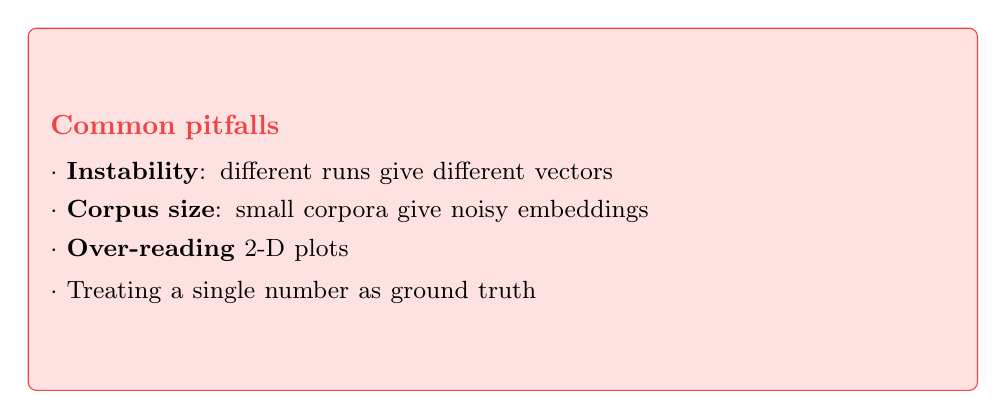
\begin{tikzpicture}
    \node[fill=warnred, draw=warnborder, rounded corners=3pt,
          inner xsep=8pt, inner ysep=8pt, text width=\columnwidth-18pt, minimum height=4.6cm]{%
      \textcolor{warnborder}{\textbf{Common pitfalls}}\\[5pt]
      {\small
      $\cdot$ \textbf{Instability}: different runs give different vectors\\[3pt]
      $\cdot$ \textbf{Corpus size}: small corpora give noisy embeddings\\[3pt]
      $\cdot$ \textbf{Over-reading} 2-D plots\\[3pt]
      $\cdot$ Treating a single number as ground truth}};
  \end{tikzpicture}

  \column{0.48\textwidth}
  \vspace{0pt}
  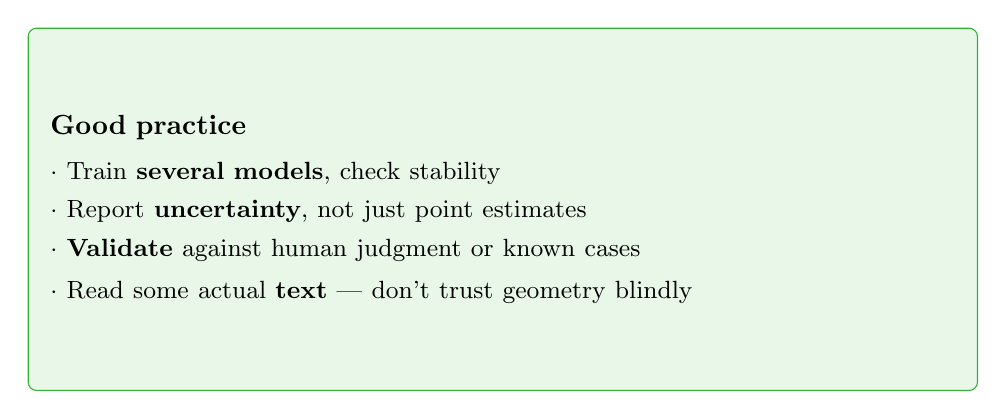
\begin{tikzpicture}
    \node[fill=lightgreen, draw=wurgreen, rounded corners=3pt,
          inner xsep=8pt, inner ysep=8pt, text width=\columnwidth-18pt, minimum height=4.6cm]{%
      \textbf{Good practice}\\[5pt]
      {\small
      $\cdot$ Train \textbf{several models}, check stability\\[3pt]
      $\cdot$ Report \textbf{uncertainty}, not just point estimates\\[3pt]
      $\cdot$ \textbf{Validate} against human judgment or known cases\\[3pt]
      $\cdot$ Read some actual \textbf{text} --- don't trust geometry blindly}};
  \end{tikzpicture}
\end{columns}

\medskip
{\small\textcolor{midgray}{\textit{The computational result is a starting point for
interpretation, not the end of it.}}}
\end{frame}

% ── SLIDE 7: Bridge - the bank problem returns ───────────────────────────────
\begin{frame}{The Limit of Static Embeddings}
\vspace{0.2cm}
{\small Static embeddings were a huge leap --- but they share one stubborn flaw with
bag-of-words. Remember ``\textbf{bank}''?}

\medskip
\begin{center}
\begin{tikzpicture}[font=\small]
  \node[fill=lightgray, rounded corners=3pt, inner sep=8pt, text width=4.7cm, align=center] (s1)
    {``I sat on the river \textbf{bank}''};
  \node[fill=lightgray, rounded corners=3pt, inner sep=8pt, text width=4.7cm, align=center, right=1.5cm of s1] (s2)
    {``I deposited cash at the \textbf{bank}''};
  \node[fill=warnred, draw=warnborder, rounded corners=3pt, inner sep=7pt,
        text width=6cm, align=center, below=0.9cm of $(s1)!0.5!(s2)$] (v)
    {\textbf{one} vector for ``bank'' --- \\ the \emph{same} in both sentences};
  \draw[-{Stealth[length=2mm]}, warnborder] (s1) -- (v);
  \draw[-{Stealth[length=2mm]}, warnborder] (s2) -- (v);
\end{tikzpicture}
\end{center}

\bigskip
{\small A static embedding gives every word \textbf{exactly one vector}, no matter the
sentence. So the two very different ``banks'' collapse into one. \textbf{Context is still
being ignored} --- just at the word level instead of the document level.}
\end{frame}

% ── SLIDE 8: Contextual embeddings intuition ─────────────────────────────────
\begin{frame}{The Fix: Contextual Embeddings}
\vspace{0.2cm}
{\small \textbf{Contextual embeddings} (BERT and its relatives) solve this: instead of one
fixed vector per word, they compute a \textbf{fresh vector for each word every time it
appears}, based on its surrounding sentence.}

\medskip
\begin{center}
\begin{tikzpicture}[font=\small]
  \node[fill=lightgreen, draw=wurgreen, rounded corners=3pt, inner sep=8pt, text width=4.7cm, align=center] (s1)
    {``river \textbf{bank}''\\$\rightarrow$ vector A};
  \node[fill=lightgreen, draw=wurgreen, rounded corners=3pt, inner sep=8pt, text width=4.7cm, align=center, right=1.5cm of s1] (s2)
    {``cash at the \textbf{bank}''\\$\rightarrow$ vector B};
  \node[text=darknavy, below=0.7cm of $(s1)!0.5!(s2)$, font=\itshape] (v)
    {vector A $\neq$ vector B --- context decides the meaning};
\end{tikzpicture}
\end{center}

\bigskip
{\small The two ``banks'' now get \textbf{different vectors}. The model reads the whole
sentence and shapes each word's representation to fit. This is the leap from \textbf{static}
to \textbf{contextual}.}
\end{frame}

% ── SLIDE 9: Attention teaser ────────────────────────────────────────────────
\begin{frame}{How? A One-Slide Peek at Attention}
\vspace{0.2cm}
{\small The engine behind contextual models is the \textbf{transformer}, and its key
mechanism is \textbf{attention}. The intuition is simple:}

\medskip
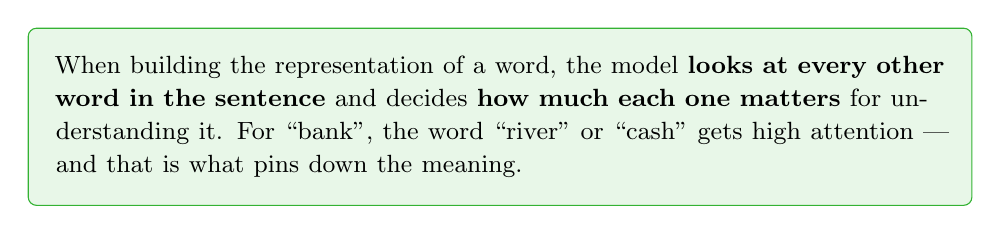
\begin{tikzpicture}
  \node[fill=lightgreen, draw=wurgreen, rounded corners=3pt,
        inner xsep=10pt, inner ysep=10pt, text width=\textwidth-24pt]{%
    {\small When building the representation of a word, the model \textbf{looks at every other
    word in the sentence} and decides \textbf{how much each one matters} for understanding it.
    For ``bank'', the word ``river'' or ``cash'' gets high attention --- and that is what
    pins down the meaning.}};
\end{tikzpicture}

\medskip
{\small That is deliberately simplified --- transformers are a course of their own. What
matters for us today: \textbf{attention is how context gets baked into every word's vector}.}

\medskip
{\small\textcolor{midgray}{\textit{We will work with these models hands-on later in the course.}}}
\end{frame}

% ── SLIDE 10: Recap ──────────────────────────────────────────────────────────
\begin{frame}{Part 2: The Takeaways}
\vspace{0.25cm}
\begin{itemize}\setlength\itemsep{8pt}
  \item[\textcolor{wurgreen}{\faCheck}]
    Embeddings \textbf{absorb social bias} from their training data --- a hazard, but also a
    \textbf{measurement opportunity}
  \item[\textcolor{wurgreen}{\faCheck}]
    Embeddings-as-measurement lets us \textbf{quantify meaning} and track it \textbf{over
    time} --- genuinely novel social science
  \item[\textcolor{wurgreen}{\faCheck}]
    They demand \textbf{careful validation}: check stability, report uncertainty, read the text
  \item[\textcolor{wurgreen}{\faCheck}]
    \textbf{Static} embeddings still give one vector per word --- context-blind at the word level
  \item[\textcolor{wurgreen}{\faCheck}]
    \textbf{Contextual} embeddings (BERT, via attention) give a vector \emph{per use} --- the
    next leap
\end{itemize}

\medskip
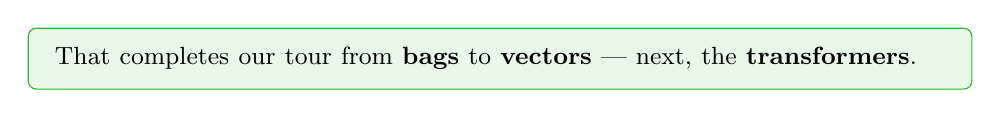
\begin{tikzpicture}
  \node[fill=lightgreen, draw=wurgreen, rounded corners=3pt,
        inner xsep=10pt, inner ysep=7pt, text width=\textwidth-24pt]{%
    {\small That completes our tour from \textbf{bags} to \textbf{vectors} --- next, the
    \textbf{transformers}.}};
\end{tikzpicture}
\end{frame}

\end{document}
